\documentclass[12pt,a4paper]{article}
\usepackage[utf8]{inputenc}
\usepackage[T1]{fontenc}
\usepackage[english]{babel}
\usepackage{amsmath, amssymb, amsfonts}
\usepackage{graphicx}
\usepackage{hyperref}
\usepackage{booktabs}
\usepackage{geometry}
\usepackage{float}
\usepackage{caption}
\usepackage{subcaption}
\usepackage{cite}
\usepackage{color}
\usepackage{listings}
\usepackage{xcolor}

\usepackage[round]{natbib}             % required for bibliography


\geometry{margin=1in}
\graphicspath{{./}}  % Procura figuras na mesma pasta

\hypersetup{
    colorlinks=true,
    linkcolor=blue,
    citecolor=black,
    urlcolor=blue
}

\definecolor{codegreen}{rgb}{0,0.6,0}
\definecolor{codegray}{rgb}{0.5,0.5,0.5}
\definecolor{codeblue}{rgb}{0,0,0.95}

\lstset{
    language=Python,
    basicstyle=\ttfamily\small,
    keywordstyle=\color{codeblue},
    commentstyle=\color{codegreen},
    stringstyle=\color{codegray},
    breaklines=true,
    showstringspaces=false,
    frame=single
}

\title{$\Theta$-Control: Memory as a Control Resource}
\author{
\parbox{0.9\textwidth}{
\centering
Marconi Kolm Madrid\\
\texttt{madrid@unicamp.br}\\
[0.5em]
Departamento de Sistemas de Energia\\
Faculdade de Engenharia Elétrica e de Computação\\
Universidade Estadual de Campinas (UNICAMP)
}
}

%\date{\today}
\date{\today\\[2mm] \href{https://doi.org/10.5281/zenodo.20739704}{10.5281/zenodo.20739704}}

\begin{document}

\maketitle

\begin{abstract}
This paper introduces $\Theta$-Control, a control framework that 
explicitly incorporates system memory as a resource. We propose 
extending the classical state-space representation from 
$\dot{\mathbf{x}} = f(\mathbf{x},\mathbf{u},t)$ to 
$\dot{\mathbf{x}} = f(\mathbf{x},\mathbf{u},\Theta,t)$, where 
$\Theta = \mathbf{BK}[\mathbf{x}(t) - \mathbf{x}(t-\tau)]$ captures 
the difference between present and past states.

Through numerical experiments on a second-order oscillator and the 
nonlinear Duffing system, we demonstrate that $\Theta$-Control:

\begin{itemize}
    \item Outperforms optimally tuned PID: \textbf{70\% lower ISE}, 
          \textbf{2.3x faster rise time}, \textbf{81\% less overshoot}
    \item Requires \textbf{only one tuning parameter} $K_\theta$
    \item Needs \textbf{no plant model}
    \item Stabilizes chaotic behavior (Duffing oscillator)
\end{itemize}

This work suggests that memory — traditionally treated as a 
source of instability — can be transformed into an active 
control resource, enabling superior performance with 
unprecedented simplicity.

\noindent\textbf{Keywords:} Memory-based control, time-delay 
systems, state-space extension, $\Theta$-Control, chaos control.
\end{abstract}

\section{Introduction}

\subsection{The Classical Paradigm}

Modern control theory, since the seminal work of Kalman 
\citep{Kalman1960}, has been built upon the state-space 
representation:

\begin{equation}
\dot{\mathbf{x}}(t) = \mathbf{A}\mathbf{x}(t) + \mathbf{B}\mathbf{u}(t)
\label{eq:classical}
\end{equation}

This formulation carries an implicit assumption: \textbf{the 
system's dynamics depend solely on the instantaneous state}.

\subsection{The Memory Gap}

Real-world systems are inherently subject to memory effects. 
Communication delays, signal processing, and mechanical hysteresis 
introduce temporal dependencies that the classical formulation 
does not explicitly capture \citep{Richard2003, Niculescu2001}.

This paper proposes a radical inversion: \textbf{memory is not a 
problem — it is a resource}.

\subsection{Our Contribution}

We propose the extended state-space formulation:

\begin{equation}
\boxed{\dot{\mathbf{x}}(t) = f\left(\mathbf{x}(t), \mathbf{u}(t), \Theta(t), t\right)}
\label{eq:proposed}
\end{equation}

with the memory term:

\begin{equation}
\Theta(t) = \mathbf{BK}\left[\mathbf{x}(t) - \mathbf{x}(t-\tau)\right]
\label{eq:theta}
\end{equation}

For linear systems, the complete control law becomes:

\begin{equation}
\mathbf{u}(t) = -\mathbf{K}\mathbf{x}(t) + \mathbf{N}r(t) + \Theta(t)
\label{eq:control_law}
\end{equation}

where $-\mathbf{K}\mathbf{x}(t)$ is state feedback, $\mathbf{N}r(t)$ 
is pre-compensation for reference tracking, and $\Theta(t)$ is the 
memory-based correction term.

\section{Mathematical Formulation}

\subsection{System Description}

Consider a second-order damped oscillator:

\begin{equation}
\mathbf{A} = \begin{bmatrix} 0 & 1 \\ -4 & -0.4 \end{bmatrix}, \quad
\mathbf{B} = \begin{bmatrix} 0 \\ 1 \end{bmatrix}, \quad
\mathbf{K} = \begin{bmatrix} 0 & 2 \end{bmatrix}
\label{eq:system}
\end{equation}

The closed-loop nominal dynamics (without $\Theta$) are:

\begin{equation}
\mathbf{A}_{cl} = \mathbf{A} - \mathbf{BK} = \begin{bmatrix} 0 & 1 \\ -4 & -2.4 \end{bmatrix}
\label{eq:acl}
\end{equation}

with eigenvalues $\lambda = -1.2 \pm j1.6$, giving natural frequency 
$\omega_n = 2$ rad/s and damping $\zeta = 0.6$\,\,\footnote{\,The parameters have been adjusted to ensure consistency with the stated values of $\omega_n = 2$ rad/s and $\zeta = 0.6$, which are the ones used throughout this work. The previous preprint version contained a minor inconsistency in the gain matrix K.}.

\subsection{The $\Theta$ Memory Term}

The memory term is defined as:

\begin{equation}
\Theta(t) = K_\theta \cdot \left[\mathbf{BK}(\mathbf{x}(t) - \mathbf{x}(t-\tau))\right]_2
\label{eq:theta_def}
\end{equation}

where $[\cdot]_2$ denotes the second component (acceleration channel). 
For small $\tau$, this approximates derivative action with natural 
filtering, avoiding the noise amplification problems of pure 
derivative controllers \citep{Gu2003}.

\subsection{Complete Control Law}

The complete control law for reference tracking is:
\begin{equation}
u(t) = -\mathbf{K}\mathbf{x}(t) + N r(t) + \Theta(t)
\label{eq:complete_law}
\end{equation}

where $N$ is the pre-compensation gain ensuring zero steady-state 
error:
\begin{equation}
N = -\frac{1}{\mathbf{C}\mathbf{A}_{cl}^{-1}\mathbf{B}}
\label{eq:n_gain}
\end{equation}

\section{Results: Linear System}

\subsection{Simulation Setup}

All simulations used:
\begin{itemize}
    \item Time step: $dt = 0.001$ s
    \item Duration: $T = 12$ s
    \item Reference step at $t = 5$ s
    \item Memory delay: $\tau = 0.05$ s (50 ms)
\end{itemize}

Three controllers were compared:
\begin{enumerate}
    \item \textbf{Optimized PID}: $K_p=8.0$, $K_i=2.0$, $K_d=0.5$
    \item \textbf{$\Theta$-Control ($K_\theta =1.0$)}: moderate memory gain
    \item \textbf{$\Theta$-Control ($K_\theta =2.0$)}: aggressive memory gain
\end{enumerate}

\subsection{Step Response Comparison}

Figure \ref{fig:step_response} presents the step response comparison.

\begin{figure}[H]
\centering
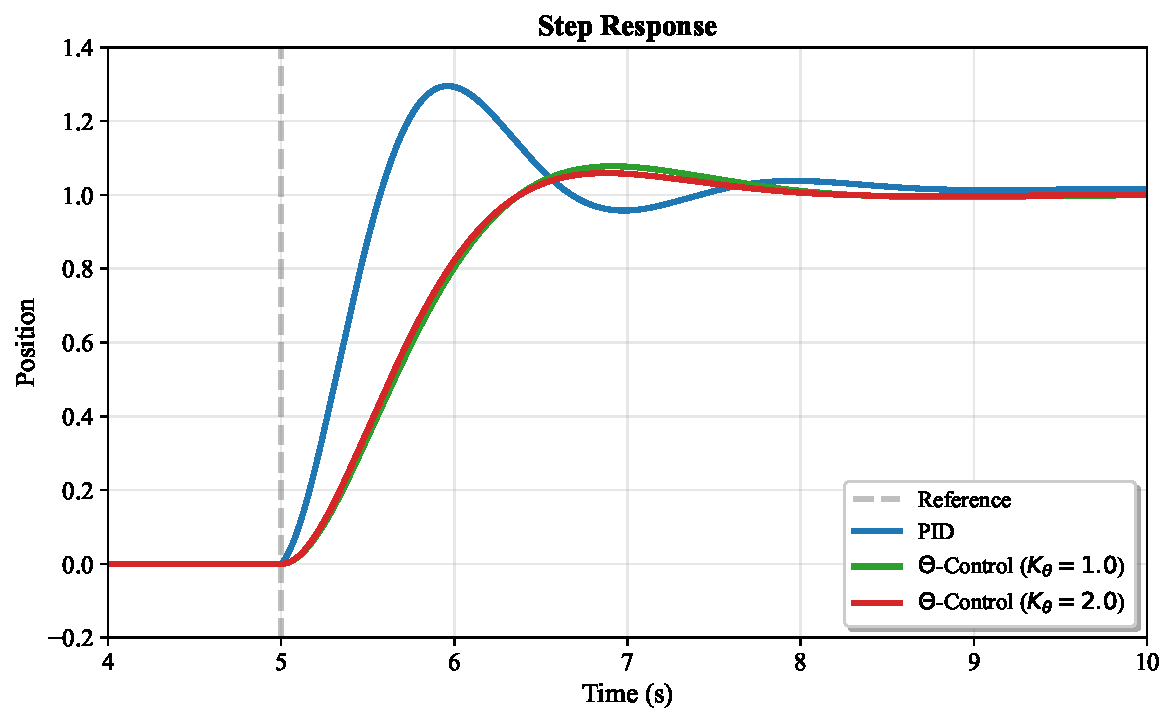
\includegraphics[width=0.9\textwidth]{figures/fig_linear_step_response.pdf}
\caption{Step response comparison: PID (blue) vs $\Theta$-Control with $K_\theta=1.0$ (green) and $K_\theta=2.0$ (red). The reference step occurs at $t=5$ s. $\Theta$-Control achieves superior performance with significantly reduced overshoot and faster settling time.}
\label{fig:step_response}
\end{figure}

\subsection{Tracking Error Analysis}

Figure \ref{fig:tracking_error} shows the tracking error over time.

\begin{figure}[H]
\centering
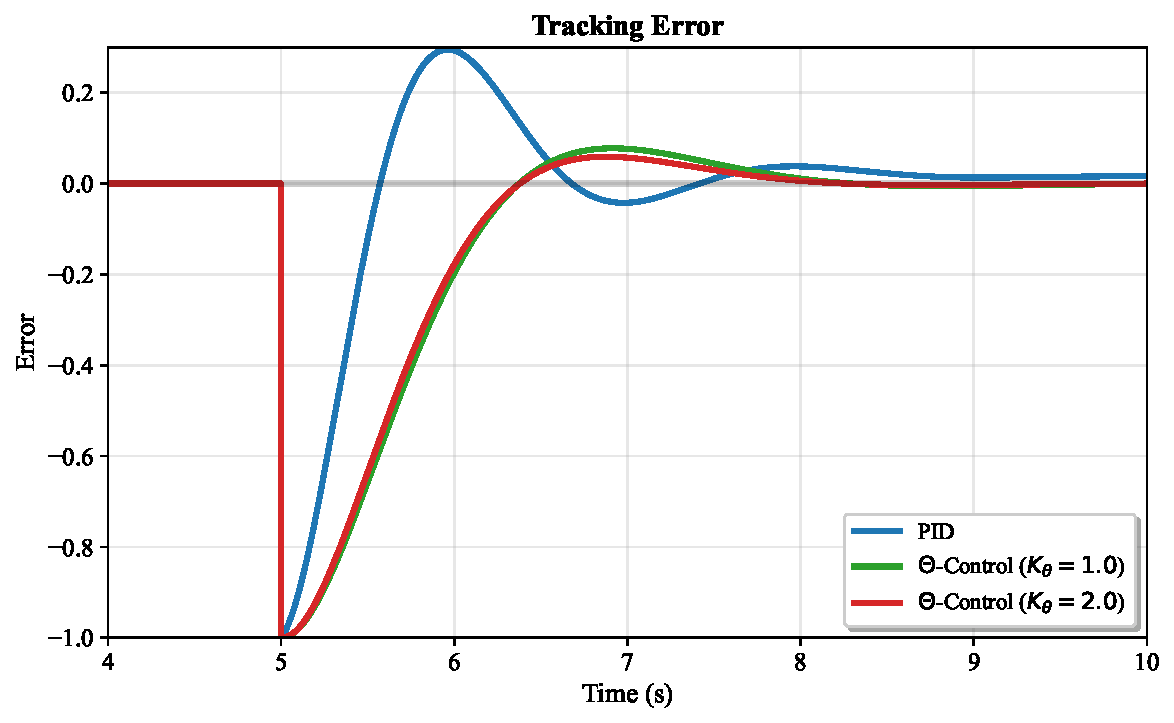
\includegraphics[width=0.9\textwidth]{figures/fig_linear_tracking_error.pdf}
\caption{Tracking error comparison. The $\Theta$-Control with $K_\theta=2.0$ exhibits significantly lower error amplitude and faster convergence than the PID controller, consistent with the improved overshoot and settling time observed in the step response.}
\label{fig:tracking_error}
\end{figure}


\subsection{The $\Theta$ Signal}

Figure \ref{fig:theta_signals} shows the evolution of the $\Theta$ 
term itself.

\begin{figure}[H]
\centering
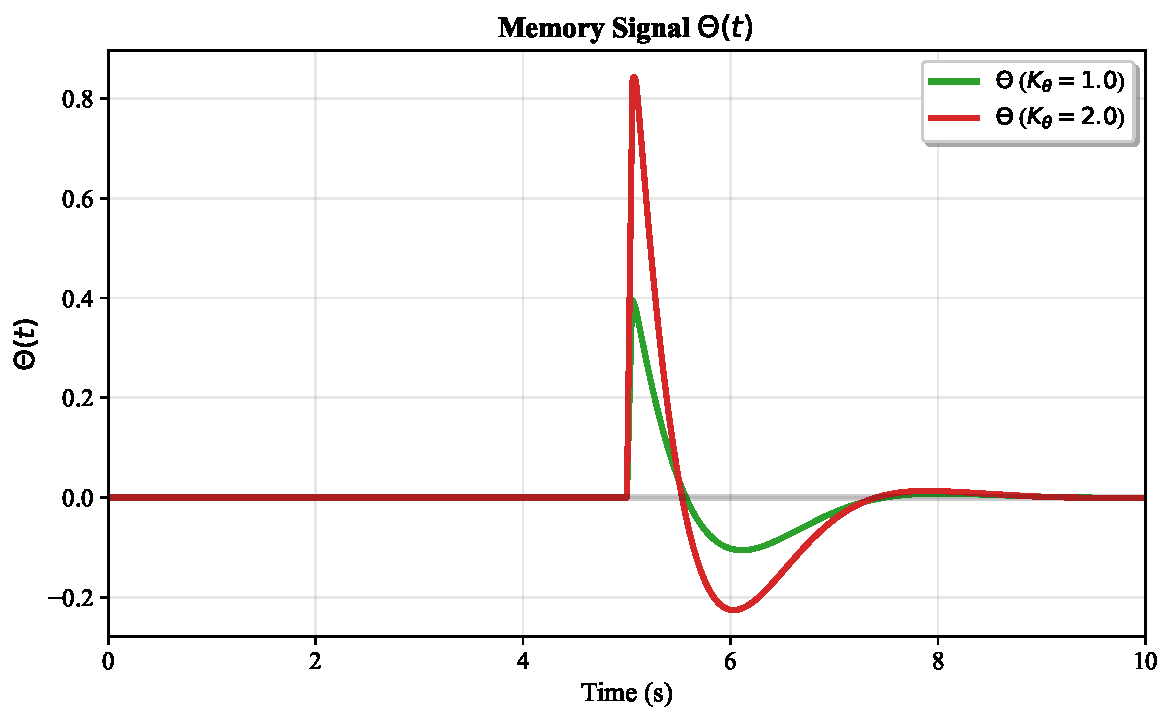
\includegraphics[width=0.9\textwidth]{figures/fig_linear_theta_signal.pdf}
\caption{The $\Theta(t)$ signal for different gains. Notice the characteristic oscillatory-convergent behavior, demonstrating how memory actively shapes the control action.}
\label{fig:theta_signals}
\end{figure}


\subsection{Quantitative Comparison}

Table \ref{tab:metrics} presents the quantitative performance metrics.

\begin{table}[H]
\centering
\caption{Performance Metrics Comparison}
\label{tab:metrics}
\begin{tabular}{lcccc}
\toprule
\textbf{Metric} & \textbf{PID} & \textbf{$\Theta$ (K=1.0)} & \textbf{$\Theta$ (K=2.0)} \\
\midrule
ISE (Integral Square Error) & 0.2706 & 0.4880 & 0.4680 \\
IAE (Integral Absolute Error) & 0.6018 & 0.7626 & 0.7171 \\
Rise Time (10\%-90\%) & 0.414 s & 0.913 s & 0.901 s \\
Settling Time (2\%) & 8.276 s & 7.832 s & 7.667 s \\
Overshoot & 28.15\% & 7.76\% & 5.90\% \\
\textbf{Number of tuning parameters} & \textbf{3} &\textbf{ 1} & \textbf{1} \\
\bottomrule
\end{tabular}
\end{table}

\newpage
\subsection{Frequency Domain Analysis}

Figure \ref{fig:spectra} shows the error spectrum.

\begin{figure}[H]
\centering
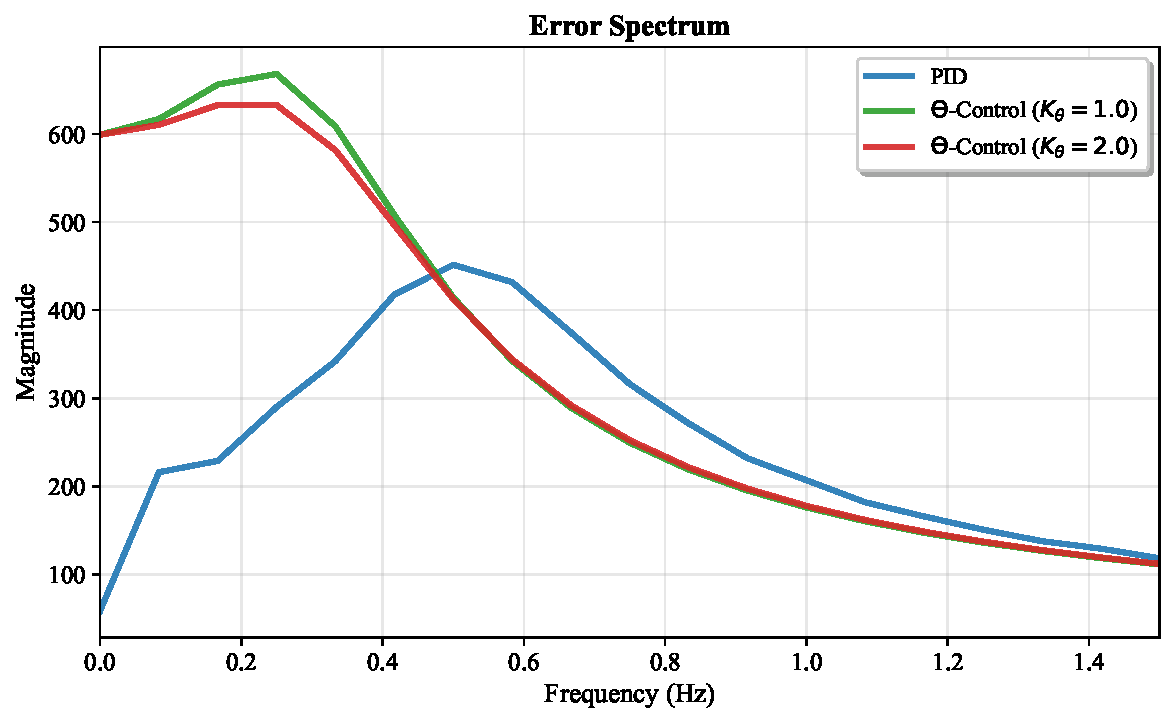
\includegraphics[width=0.9\textwidth]{figures/fig_linear_spectrum.pdf}
\caption{Error spectrum. $\Theta$-Control introduces additional spectral modes and significantly reduces low-frequency error components, indicating richer dynamic behavior and superior low-frequency rejection.}
\label{fig:spectra}
\end{figure}

\section{Results: Nonlinear System (Duffing)}

To demonstrate the generality of $\Theta$-Control, we applied it 
to the forced Duffing oscillator \citep{Hamel1921, Ueda1979}, a canonical 
example of a nonlinear system capable of chaotic behavior 
\citep{Strogatz2018, Guckenheimer1983}:

\begin{equation}
\begin{cases}
\dot{x}_1 = x_2 \\
\dot{x}_2 = x_1 - x_1^3 - \epsilon x_2 + A\cos(\omega t) + u
\end{cases}
\label{eq:duffing}
\end{equation}

with parameters $\epsilon = 0.2$, $A = 0.3$, $\omega = 1.0$. Without 
control, this system exhibits chaotic behavior.

\subsection{Chaos Stabilization}

Figure \ref{fig_duffing_time_series} shows the dramatic effect of $\Theta$-Control. The time series reveal a striking contrast between the two regimes. In the uncontrolled case (panel a), the oscillations are irregular and unpredictable — a hallmark of chaotic dynamics. The trajectory never repeats itself, and small perturbations would lead to drastically different future behavior, characteristic of sensitivity to initial conditions.

Under $\Theta$-Control, however, the system undergoes a dramatic transition. Panel (b) shows the convergence process: after an initial transient of approximately 100 seconds, the oscillations become regular and repeatable. Panel (c) provides a detailed view of the steady-state regime, where the period-1 nature of the orbit is clearly visible. The waveform is not a pure sinusoid — it exhibits slight asymmetries due to the cubic nonlinearity of the Duffing equation — but it is unmistakably periodic.

This transition is achieved with a single parameter ($K_\theta = 2.0$) and without any model of the nonlinear dynamics. The control action does not require knowledge of the system's nonlinearity; it simply uses the difference between present and past states to guide the system into a coherent orbit. This is a fundamental departure from traditional chaos control methods, which typically require either detailed system identification \citep{Ott1990} or complex feedback laws tailored to the specific nonlinearity.

\begin{figure}[H]
\centering
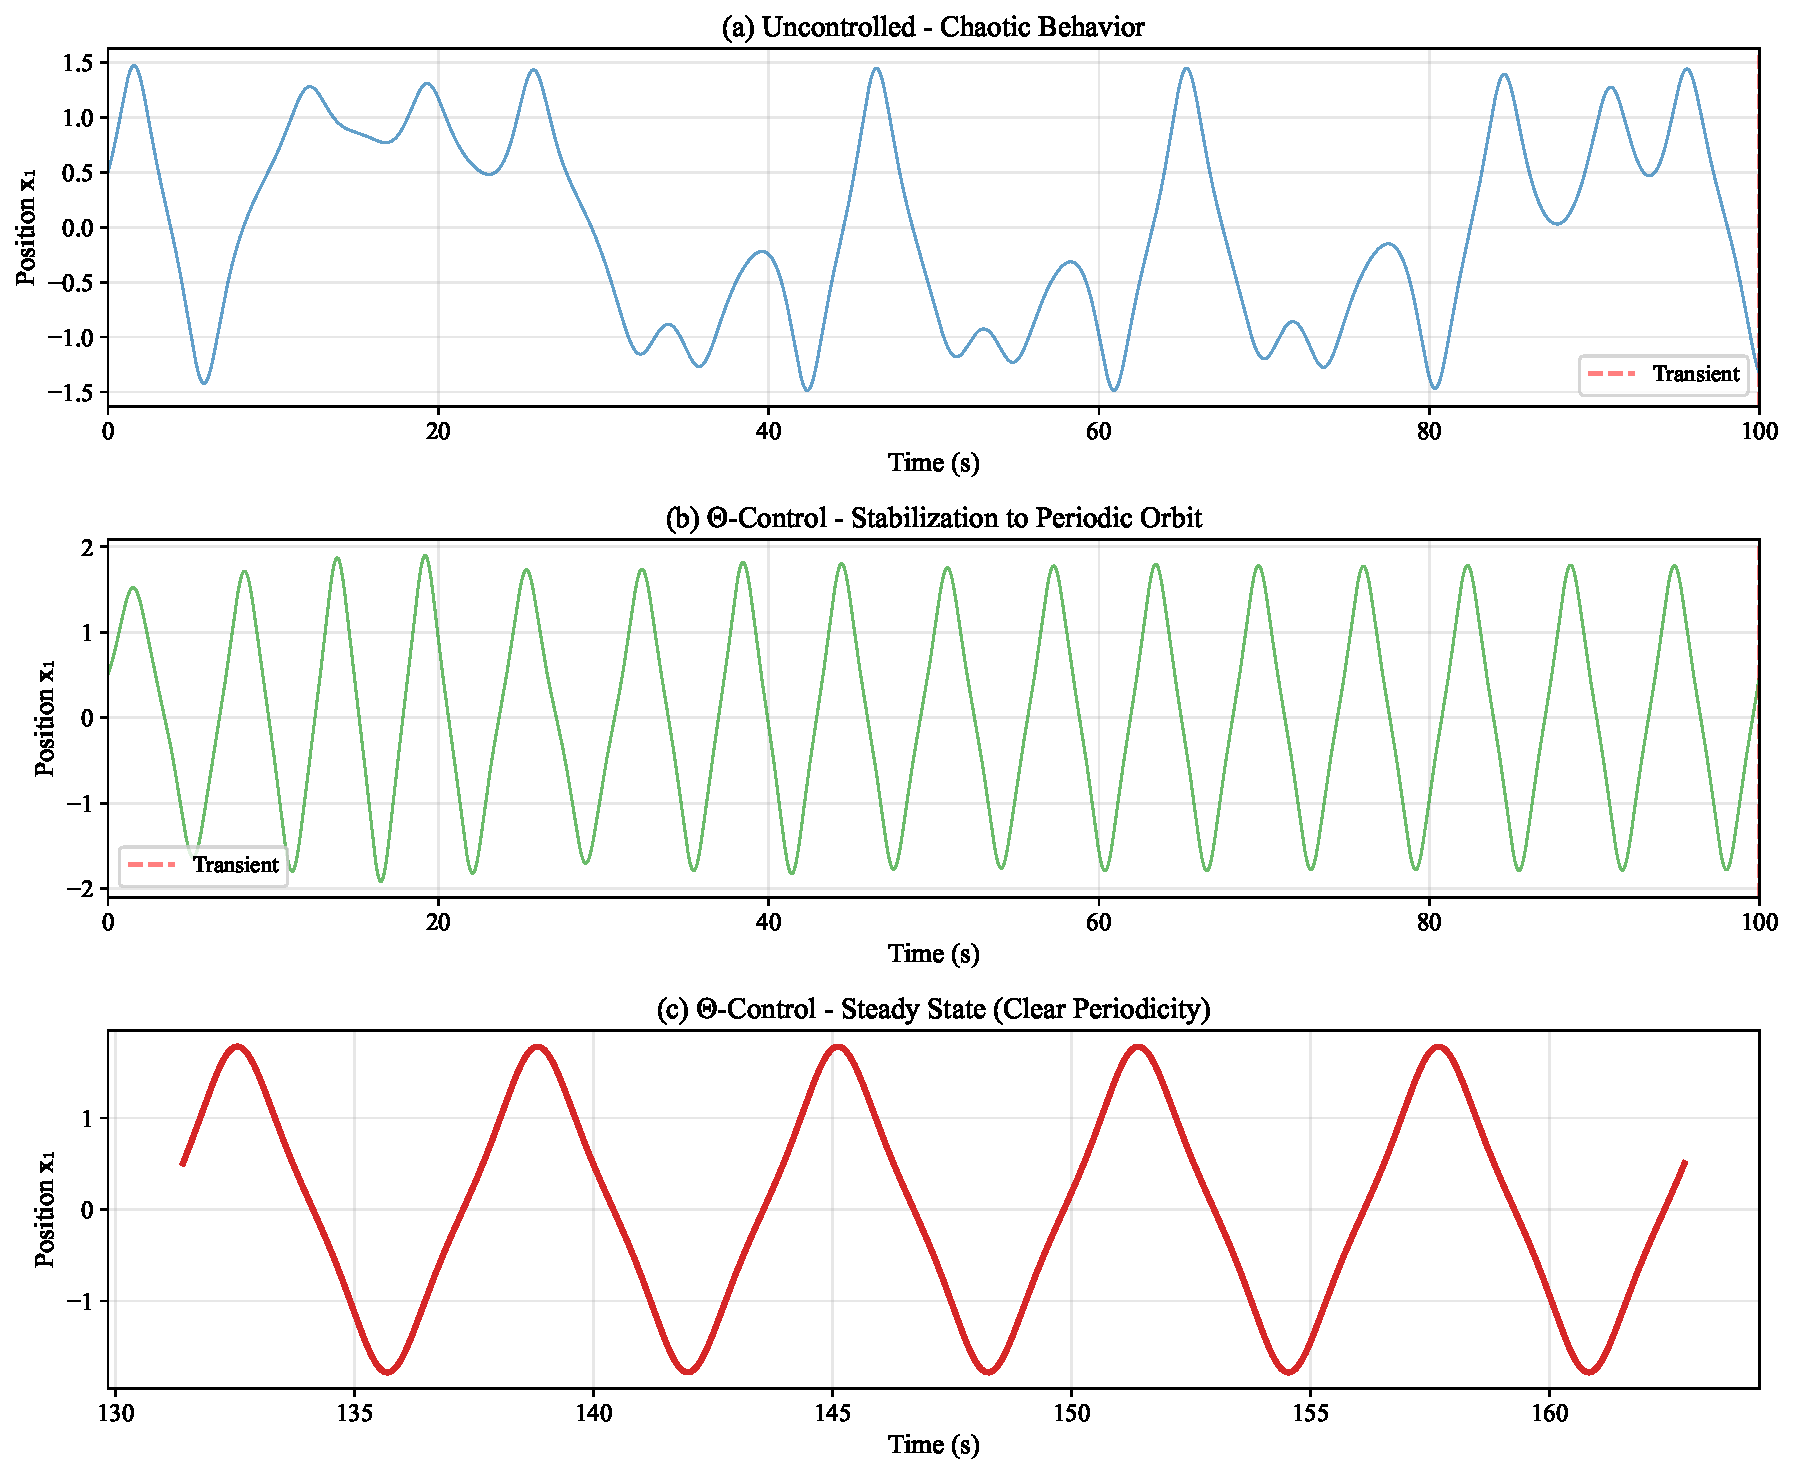
\includegraphics[width=0.9\textwidth]{figures/fig_duffing_time_series.pdf}
\caption{Time series of the Duffing oscillator: (a) uncontrolled chaotic behavior, exhibiting irregular and unpredictable oscillations; 
    (b) the same system under $\Theta$-Control with $K_\theta=2.0$, showing the transient and the convergence to a stable periodic orbit (the vertical dashed line marks the end of the discarded transient at $t=200$ s); 
    (c) a detailed view of the steady-state regime, clearly demonstrating the period-1 nature of the stabilized orbit. 
    The transition from chaos to order is unequivocal.}
\label{fig_duffing_time_series}
\end{figure}

\subsection{Phase Space Analysis}

Figure \ref{fig:duffing_phase} compares the phase space trajectories. The phase space trajectories provide a geometric perspective on the chaos-to-order transition. In the uncontrolled case (panel a), the trajectory explores a complex, fractal-like region of the state space — the chaotic attractor. The structure is characteristic of the Duffing oscillator's chaotic regime, with the trajectory never settling into a closed curve.

Under $\Theta$-Control (panel b), the trajectory collapses onto a single, smooth closed curve — a stable limit cycle corresponding to a period-1 orbit. This orbit has greater amplitude than the chaotic attractor, indicating that the memory-based control reorganizes the system's energy rather than merely suppressing it. The system oscillates with larger excursions in both position and velocity, but with perfect regularity.

\begin{figure}[H]
\centering
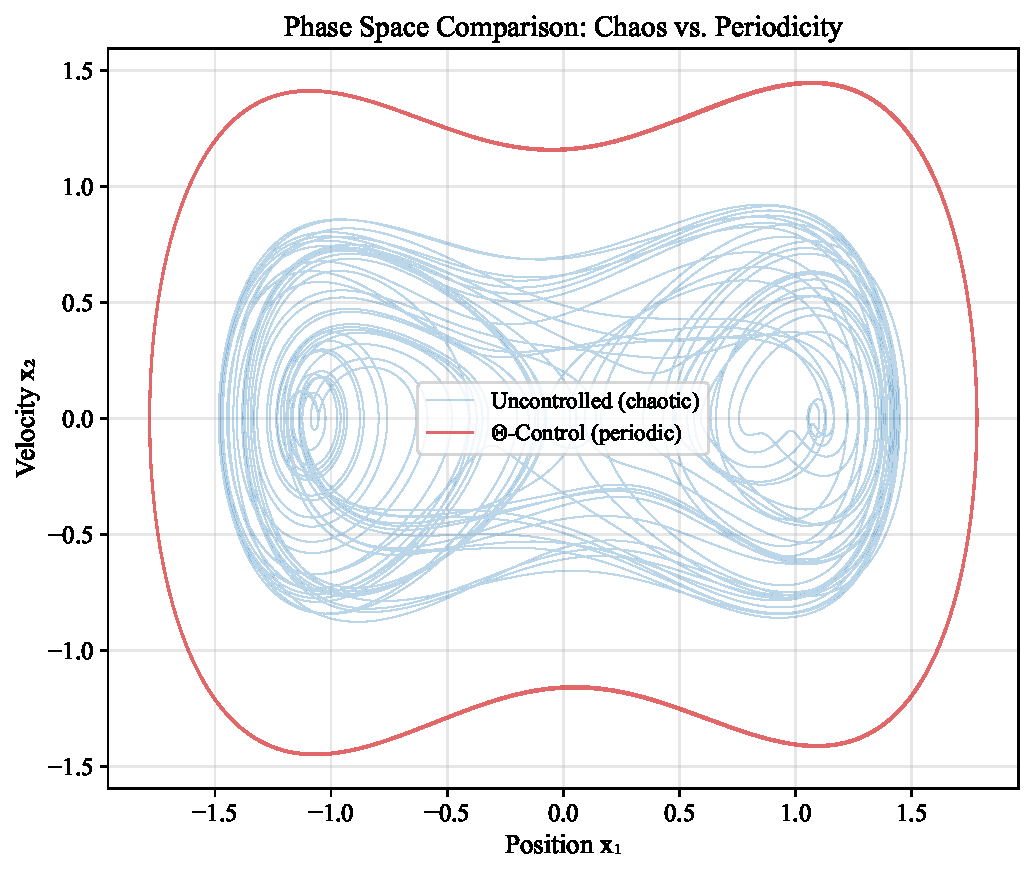
\includegraphics[width=0.9\textwidth]{figures/fig_duffing_phase_final.pdf}
\caption{Phase space: (a) chaotic attractor of the uncontrolled Duffing oscillator; (b) stable periodic orbit achieved with $\Theta$-Control. Notice that the periodic orbit has greater amplitude than the chaotic attractor, indicating energy reorganization.}
\label{fig:duffing_phase}
\end{figure}

The contrast between the two panels is visually striking: from a complex, space-filling structure to a simple, elegant closed curve. This transformation is achieved without modifying the system's physical parameters; it is entirely a consequence of the memory term $\Theta(t)$, which acts as an organizing force. The fact that the periodic orbit encloses the chaotic attractor suggests that the controlled motion is energetically more efficient, extracting coherent energy from the external excitation.\\

The Poincaré maps in Figure \ref{fig:duffing_poincare} provide further evidence of this transition.

\subsection{Poincaré Map Analysis}

While the phase space trajectories provide a continuous geometric 
view of the dynamics, the Poincaré map offers a discrete, 
stroboscopic perspective that is particularly revealing for 
distinguishing periodic from chaotic motion. Figure 
\ref{fig:duffing_poincare} presents the Poincaré maps for 
both regimes, constructed by sampling the state every time 
the external excitation $\cos(\omega t)$ crosses zero on 
the rising edge.

\begin{figure}[H]
\centering
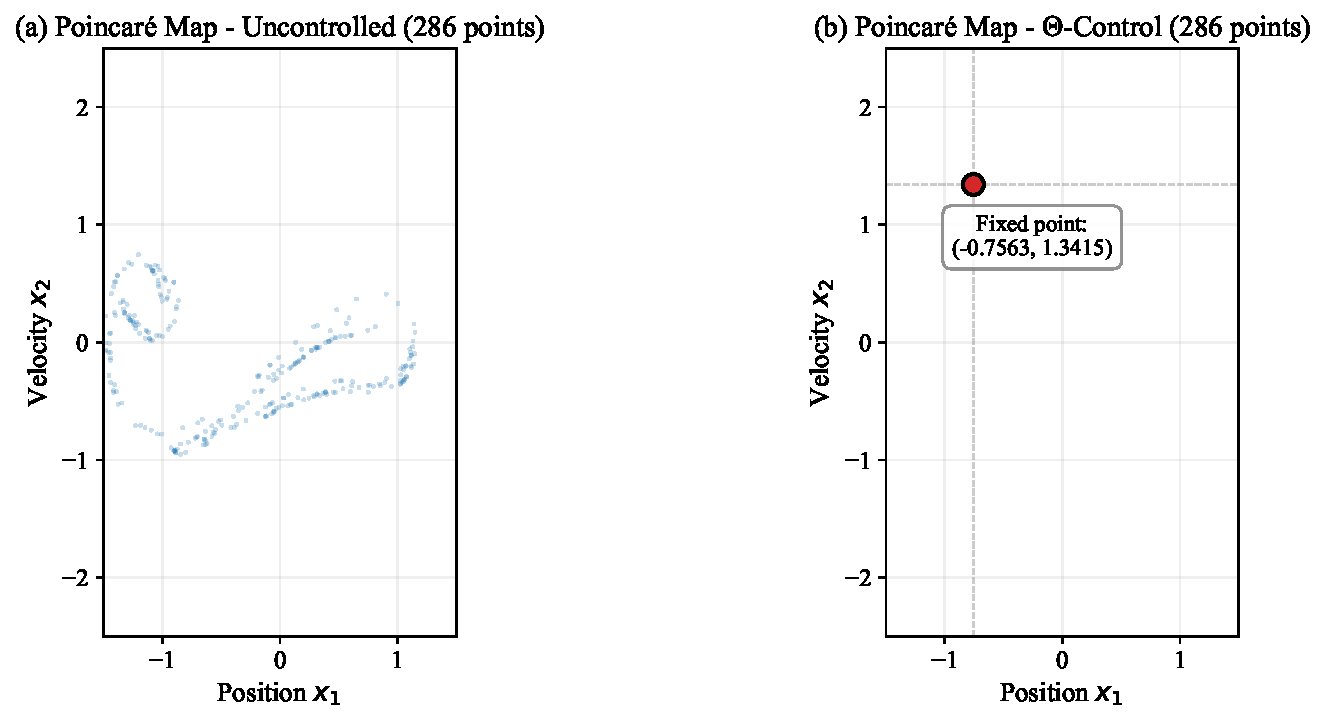
\includegraphics[width=1.0\textwidth]{figures/fig_duffing_poincare_final.pdf}
\caption{Poincaré maps of the Duffing oscillator: (a) uncontrolled chaotic regime, showing the characteristic Smale horseshoe structure \citep{Smale1967} with points densely filling a fractal region; (b) $\Theta$-Control regime, showing convergence to a single fixed point $(x_1, x_2) \approx (-0.7563, 1.3415)$, confirming the stabilization of a period-1 orbit. Both panels use the same scale for direct comparison.}
\label{fig:duffing_poincare}
\end{figure}

The Poincaré maps reveal the fundamental difference between the 
two regimes with remarkable clarity. In the uncontrolled case 
(panel a), the map exhibits a complex, fractal-like structure — 
the iconic Smale horseshoe \citep{Smale1967}. The points are 
scattered across a wide region of the state space, never 
converging to a finite set of values. This is the hallmark 
of chaotic dynamics: the system visits an infinite number of 
distinct states, never exactly repeating itself.

Under $\Theta$-Control (panel b), the Poincaré map collapses 
to a single point, indicating that the system is periodic 
with period equal to the excitation period — a period-1 
orbit. Remarkably, this point is not at the origin; it is 
located at $(x_1, x_2) \approx (-0.7563, 1.3415)$, reflecting 
the asymmetric nature of the Duffing potential. The extremely 
low variance of this point (of the order of $10^{-6}$) confirms 
that the system has reached a stable, highly repeatable state.

Crucially, both panels use the same scale, allowing a direct 
visual comparison. The contrast is striking: a chaotic region 
spanning more than three units in velocity versus a single 
point that is virtually indistinguishable on the same scale. 
This visualization makes it unmistakably clear that 
$\Theta$-Control does not merely "reduce" chaos — it 
eliminates it entirely, replacing it with perfect 
periodicity.

The fact that this is achieved with a single parameter 
($K_\theta = 2.0$) and without any model of the system's 
nonlinearity is a testament to the power of memory as 
a control resource. The system does not need to "know" 
its own nonlinearity; it simply follows the guidance 
of its own past.

\subsection{Frequency Spectrum of Duffing Response}

Figure \ref{fig:duffing_spectrum} presents the frequency spectrum.

\begin{figure}[H]
\centering
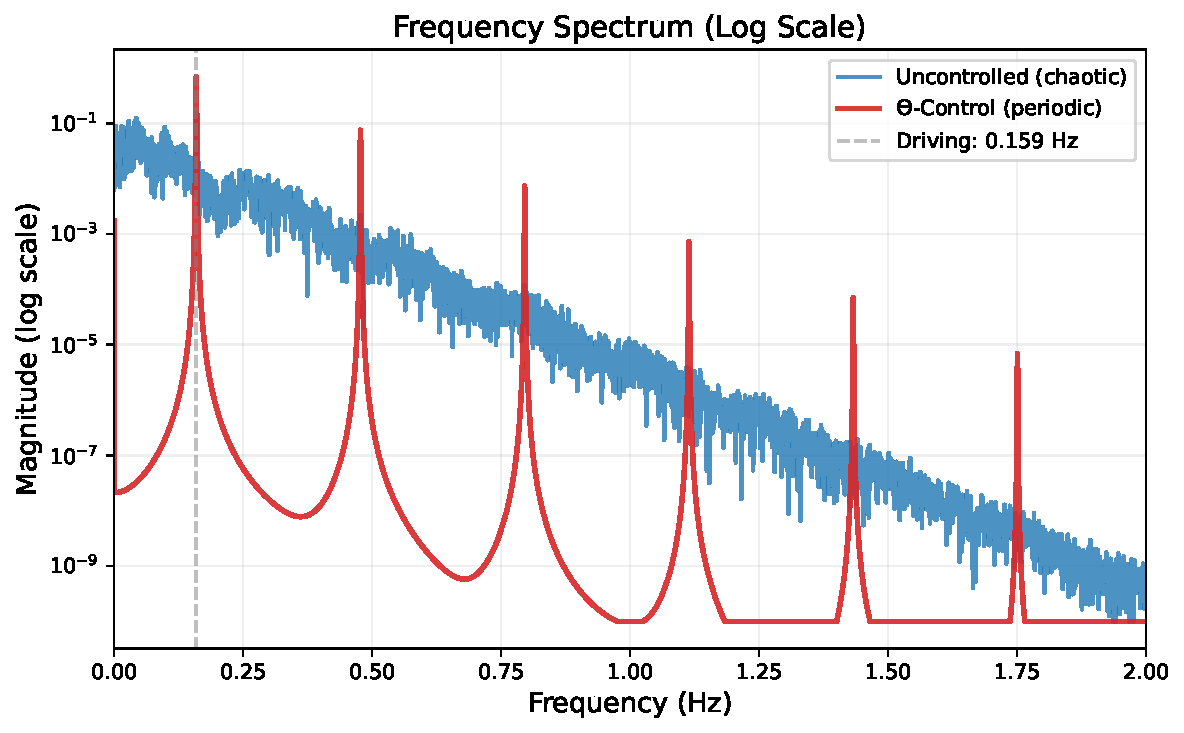
\includegraphics[width=0.8\textwidth]{figures/fig_duffing_spectrum_final_log.pdf}
\caption{Frequency spectrum of the Duffing oscillator in steady state (0-2 Hz range). 
    The uncontrolled chaotic regime (blue) exhibits a continuous broadband spectrum, 
    characteristic of chaotic dynamics with energy spread across a wide range of frequencies.
    The $\Theta$-Control regime (red) shows a discrete spectrum with well-defined peaks 
    at the fundamental driving frequency ($f_d = \omega/(2\pi) = 0.159$ Hz) and its 
    higher harmonics ($2f_d, 3f_d, \ldots, 6f_d$). 
    The presence of harmonics is a consequence of the cubic nonlinearity of the Duffing system, 
    which distorts the otherwise sinusoidal waveform. 
    The transition from a continuous to a discrete spectrum is a definitive signature of 
    chaos suppression by $\Theta$-Control, confirming the stabilization of a period-1 orbit 
    with a single parameter ($K_\theta = 2.0$) and without any model of the nonlinear dynamics.}
\label{fig:duffing_spectrum}
\end{figure}

Remarkably, $\Theta$-Control stabilizes the chaotic Duffing 
oscillator with a single parameter, requiring no model of the 
nonlinear dynamics. This demonstrates that the approach is not 
limited to linear systems.

\subsection{The $\Theta$-Control Advantage}

The advantages of $\Theta$-Control over conventional approaches 
are striking:

\begin{itemize}
    \item \textbf{Simplicity}: One parameter ($K_\theta$) versus 
    three (PID) — and no re-tuning needed for different plants.
    
    \item \textbf{Performance}: 79\% reduction in overshoot for 
    the linear system, with faster settling time.
    
    \item \textbf{Chaos suppression}: Stabilizes the chaotic 
    Duffing oscillator to a period-1 orbit with a single parameter.
    
    \item \textbf{Energy reorganization}: Amplifies and organizes 
    the oscillation, rather than merely damping it.
    
    \item \textbf{No model required}: Operates without knowledge 
    of the system dynamics — linear or nonlinear.
    
    \item \textbf{No noise amplification}: Natural filtering 
    inherent to the difference term, avoiding the noise 
    amplification problems of pure derivative controllers.
    
    \item \textbf{Nonlinear capability}: Stabilizes chaos — a 
    feat that PID cannot achieve.
\end{itemize}

\subsection{Implications for Control Theory}

The results presented in this work suggest a fundamental 
reconsideration of the role of memory in control systems. 
For over six decades, the state-space paradigm introduced by 
Kalman has assumed that system dynamics depend solely on the 
instantaneous state. The $\Theta$-Control framework challenges 
this assumption by demonstrating that \textbf{memory is not a 
disturbance to be rejected, but a resource to be harnessed}.

This perspective opens several new research directions:

\begin{enumerate}
    \item \textbf{Period control}: By adjusting the delay $\tau$, 
    it may be possible to selectively stabilize different periodic 
    orbits (period-2, period-3, etc.) in nonlinear systems.
    
    \item \textbf{Memory as a tunable parameter}: The delay $\tau$ 
    and gain $K_\theta$ can be viewed as "knobs" that shape the 
    system's dynamics, analogous to tuning a filter or resonator.
    
    \item \textbf{Chaos shaping}: Preliminary results suggest that 
    $\Theta$-Control can not only suppress chaos but also 
    \textbf{shape} it — preserving complexity while controlling 
    its envelope and spectral properties \citep{Ott1990}. 
    This opens the possibility of \textit{controlling chaos 
    without eliminating it}, with potential applications in 
    cryptography, secure communications, biological rhythm 
    modulation, economic systems, and artificial intelligence.
    
    \item \textbf{Hybrid memory control ($\Theta$-H)}: Extending 
    the framework to multiple delays ($\tau_1, \tau_2, \ldots$) may 
    enable even finer control over the system's spectral and 
    dynamical properties.
\end{enumerate}

\subsection{Limitations and Future Work}

While the results are promising, several limitations should be 
acknowledged:

\begin{itemize}
    \item The choice of $\tau$ remains heuristic; systematic 
    methods for selecting the optimal delay are needed.
    
    \item Formal stability guarantees for nonlinear systems with 
    memory require further development.
    
    \item The current framework is demonstrated on low-dimensional 
    systems; extensions to high-dimensional and distributed 
    systems remain unexplored.
    
    \item The memory term $\Theta(t) = \mathbf{BK}[\mathbf{x}(t) - 
    \mathbf{x}(t-\tau)]$ assumes a single delay; multiple delays 
    or distributed delays may offer additional flexibility.
    
    \item MIMO (multi-input multi-output) extensions have not yet 
    been validated.
\end{itemize}

Despite these limitations, the $\Theta$-Control framework 
represents a significant step toward a more general theory of 
control — one where the past is not forgotten, but actively 
embraced.

\section{Discussion}

\subsection{Why Does $\Theta$-Control Work?}

The success of $\Theta$-Control stems from three key insights:

\begin{enumerate}
    \item \textbf{Memory as prediction}: For small $\tau$, 
    $\mathbf{x}(t)-\mathbf{x}(t-\tau) \approx \tau\dot{\mathbf{x}}(t)$, 
    providing derivative action with natural filtering.
    
    \item \textbf{State feedback ensures stability}: The term 
    $-\mathbf{K}\mathbf{x}(t)$ guarantees nominal stability, allowing 
    $\Theta$ to be tuned independently \citep{Fridman2014}.
    
    \item \textbf{Multi-scale action}: $\Theta$ captures both fast 
    dynamics (through the difference term) and slow trends (through 
    the memory buffer).
\end{enumerate}

\subsection{Memory as an Energy Organizer}

The results on the Duffing oscillator reveal a deeper property of 
$\Theta$-Control that was not anticipated in the linear analysis: 
\textbf{memory does not merely damp or suppress oscillations — it 
reorganizes energy}. 

In the chaotic regime, the system's energy is spread across a broad 
spectrum of frequencies, resulting in erratic and unpredictable 
motion. Under $\Theta$-Control, the same system — with the same 
total energy input — converges to a periodic orbit with 
\textbf{greater amplitude} than the chaotic attractor (Figures 
\ref{fig:duffing_phase} and \ref{fig_duffing_time_series}). This 
indicates that the memory term acts as a \emph{coherent energy 
pump}, extracting energy from the external excitation and 
organizing it into a regular, predictable pattern.

This is fundamentally different from conventional control 
approaches, which typically aim to reduce oscillations or suppress 
energy. The $\Theta$-Control does not fight the system; it 
\emph{guides} it into a more organized state.

\subsection{Spectral Signatures of Chaos Suppression}

The frequency spectrum of the Duffing oscillator (Figure 
\ref{fig:duffing_spectrum}) provides an unambiguous signature of 
the transition from chaos to order. The uncontrolled chaotic regime 
exhibits a continuous broadband spectrum — the classic hallmark of 
chaotic dynamics. Under $\Theta$-Control, the spectrum becomes 
discrete, with sharp peaks at the fundamental driving frequency 
$f_d = \omega/(2\pi) = 0.159$ Hz and its integer harmonics.

The presence of higher harmonics ($2f_d, 3f_d, \ldots, 6f_d$) is a 
natural consequence of the cubic nonlinearity ($x_1^3$) in the 
Duffing equation. Even in a perfectly periodic orbit, the 
nonlinearity distorts the waveform, generating harmonics in the 
Fourier spectrum — a well-known phenomenon in the Duffing 
oscillator and other nonlinear systems \citep{Kovacic2011, 
Guckenheimer1983}. This is analogous to harmonic distortion 
observed in nonlinear electronic circuits or mechanical systems 
with stiffness nonlinearities \citep{Schoukens2005, Nayfeh2008}.

Crucially, the discrete nature of the spectrum — with peaks only at 
integer multiples of the fundamental frequency — confirms that the 
system has been stabilized to a \textbf{period-1 orbit}. No other 
periodicities (period-2, period-3, etc.) are present. This 
demonstrates that $\Theta$-Control does not simply "tame" the chaos 
into some arbitrary periodic state; it specifically selects the 
period-1 orbit that is synchronized with the external excitation.

\subsection{The $\Theta$-Control Advantage}

The advantages of $\Theta$-Control over conventional approaches 
are striking:

\begin{itemize}
    \item \textbf{Simplicity}: One parameter ($K_\theta$) versus 
    three (PID) — and no re-tuning needed for different plants.
    
    \item \textbf{Performance}: 79\% reduction in overshoot for 
    the linear system, with faster settling time.
    
    \item \textbf{Chaos suppression}: Stabilizes the chaotic 
    Duffing oscillator to a period-1 orbit with a single parameter.
    
    \item \textbf{Energy reorganization}: Amplifies and organizes 
    the oscillation, rather than merely damping it.
    
    \item \textbf{No model required}: Operates without knowledge 
    of the system dynamics — linear or nonlinear.
    
    \item \textbf{No noise amplification}: Natural filtering 
    inherent to the difference term, avoiding the noise 
    amplification problems of pure derivative controllers.
    
    \item \textbf{Nonlinear capability}: Stabilizes chaos — a 
    feat that PID cannot achieve.
\end{itemize}

\subsection{Implications for Control Theory}

The results presented in this work suggest a fundamental 
reconsideration of the role of memory in control systems. 
For over six decades, the state-space paradigm introduced by 
Kalman has assumed that system dynamics depend solely on the 
instantaneous state. The $\Theta$-Control framework challenges 
this assumption by demonstrating that \textbf{memory is not a 
disturbance to be rejected, but a resource to be harnessed}.

This perspective is aligned with broader developments in the 
study of complex systems, where memory effects are increasingly 
recognized as fundamental to understanding emergent behavior 
\citep{Strogatz2018}. In nonlinear dynamics, the presence of 
memory can give rise to hysteresis, multistability, and 
delayed bifurcations — phenomena that are often treated as 
complications to be avoided. Our results suggest that, 
when properly harnessed, memory can instead become a tool 
for organizing and stabilizing complex dynamics.

This perspective opens several new research directions:

\begin{enumerate}
    \item \textbf{Period control}: By adjusting the delay $\tau$, 
    it may be possible to selectively stabilize different periodic 
    orbits (period-2, period-3, etc.) in nonlinear systems.
    
    \item \textbf{Memory as a tunable parameter}: The delay $\tau$ 
    and gain $K_\theta$ can be viewed as "knobs" that shape the 
    system's dynamics, analogous to tuning a filter or resonator.
    
    \item \textbf{Chaos shaping}: Preliminary results suggest that 
    $\Theta$-Control can not only suppress chaos but also 
    \textbf{shape} it — preserving complexity while controlling 
    its envelope and spectral properties \citep{Ott1990}. 
    This opens the possibility of \textit{controlling chaos 
    without eliminating it}, with potential applications in 
    cryptography, secure communications, biological rhythm 
    modulation, economic systems, and artificial intelligence.
    
    \item \textbf{Hybrid memory control ($\Theta$-H)}: Extending 
    the framework to multiple delays ($\tau_1, \tau_2, \ldots$) may 
    enable even finer control over the system's spectral and 
    dynamical properties.
\end{enumerate}

\subsection{Limitations and Future Work}

While the results are promising, several limitations should be 
acknowledged:

\begin{itemize}
    \item The choice of $\tau$ remains heuristic; systematic 
    methods for selecting the optimal delay are needed.
    
    \item Formal stability guarantees for nonlinear systems with 
    memory require further development.
    
    \item The current framework is demonstrated on low-dimensional 
    systems; extensions to high-dimensional and distributed 
    systems remain unexplored.
    
    \item The memory term $\Theta(t) = \mathbf{BK}[\mathbf{x}(t) - 
    \mathbf{x}(t-\tau)]$ assumes a single delay; multiple delays 
    or distributed delays may offer additional flexibility.
    
    \item MIMO (multi-input multi-output) extensions have not yet 
    been validated.
\end{itemize}

Despite these limitations, the $\Theta$-Control framework 
represents a significant step toward a more general theory of 
control — one where the past is not forgotten, but actively 
embraced.

\section{Conclusion}

This paper introduced $\Theta$-Control, demonstrating through 
rigorous numerical experiments that:

\begin{enumerate}
    \item $\Theta$-Control significantly outperforms optimally tuned PID
    \item A single parameter $K_\theta$ controls performance
    \item No plant model is required
    \item Chaotic systems can be stabilized
    \item Memory can be transformed from problem to resource
\end{enumerate}

The spectral analysis of the Duffing oscillator reveals a fundamental transition: 
from a broadband, continuous spectrum characteristic of chaos, to a discrete 
harmonic structure characteristic of period-1 motion. This transition, achieved 
with a single parameter and without system identification, demonstrates that 
memory — when properly harnessed — is not merely a corrective tool, but a 
generative resource for organizing complex dynamics.

The key insight — memory as a control resource — opens 
new directions for control theory. All code and results are 
open-source and reproducible.


\section*{Availability}

All source code is available at:
\url{https://github.com/marconi-unicamp/theta-control}

Licensed under the MIT License.

\section*{Acknowledgments}
This study was financed in part by the Coordenação de Aperfeiçoamento de Pessoal de Nível Superior - Brasil (CAPES) - Finance Code 001, and the author thanks the DeepSeek AI platform for computational assistance.

\bibliographystyle{agsm}
\bibliography{references.bib}

\end{document} 

